% Two representative wires per party: retained (outer) and measured (inner).
% Smooth links connect paired qubits; double-line arrows carry classical outcomes.
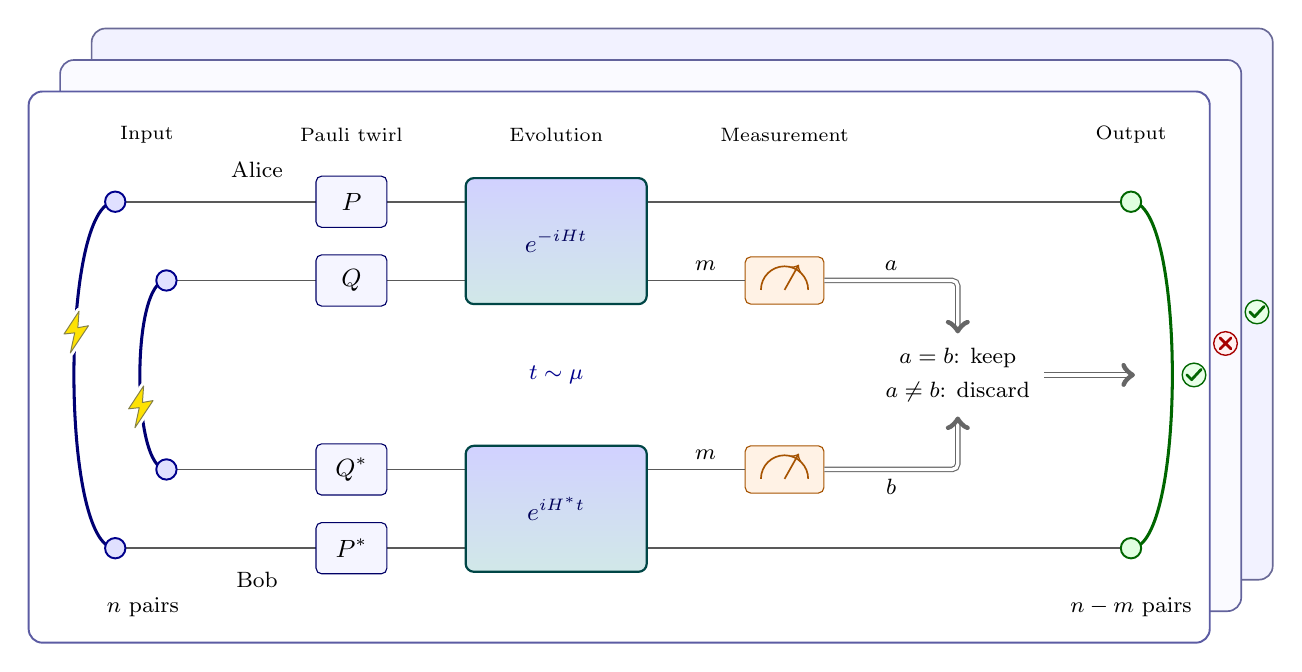
\begin{tikzpicture}[
    x=1cm,y=1cm,font=\small,
    gate/.style={draw=blue!40!black,fill=blue!4,rounded corners=2pt,
        minimum height=6.5mm,minimum width=9mm,align=center},
    evolution/.style={draw=teal!55!black,rounded corners=3pt,
        left color=blue!18!white,right color=teal!18!white,
        shading angle=0,line width=.8pt,text=blue!35!black,
        minimum height=16mm,minimum width=23mm,align=center},
    measure/.style={draw=orange!65!black,fill=orange!10,
        rounded corners=2pt,minimum width=10mm,minimum height=6mm},
    wire/.style={draw=black!65,line width=.65pt},
    classical/.style={draw=black!60,double=white,double distance=1.2pt,line width=.4pt},
    entanglement/.style={line width=1.1pt,line cap=round},
    heading/.style={font=\scriptsize},
    qubit/.style={circle,draw=blue!55!black,fill=blue!12,
        line width=.7pt,inner sep=2.6pt}
]
    % A shallow stack represents independently processed groups of n pairs.
    % Draw back to front; only narrow top and right margins remain visible.
    \path[draw=blue!18!gray,fill=blue!5,rounded corners=5pt,line width=.6pt]
        (-.3,-2.6) rectangle (14.7,4.4);
    \path[draw=blue!22!gray,fill=blue!2,rounded corners=5pt,line width=.6pt]
        (-.7,-3) rectangle (14.3,4);
    \path[draw=blue!28!gray,fill=white,rounded corners=5pt,line width=.7pt]
        (-1.1,-3.4) rectangle (13.9,3.6);

    % Outcome badges occupy the same position relative to each card:
    % just beyond the output pair, halfway between Alice and Bob.
    \foreach \x/\y in {13.7/0,14.5/.8} {
        \begin{scope}[shift={(\x,\y)}]
            \path[fill=green!9,draw=green!40!black,line width=.5pt]
                (0,0) circle[radius=.15];
            \draw[draw=green!40!black,line width=1pt,line cap=round,line join=round]
                (-.09,0) -- (-.03,-.06) -- (.09,.07);
        \end{scope}
    }
    \begin{scope}[shift={(14.1,.4)}]
        \path[fill=red!6,draw=red!65!black,line width=.5pt]
            (0,0) circle[radius=.15];
        \draw[draw=red!65!black,line width=1pt,line cap=round]
            (-.07,-.07) -- (.07,.07)
            (-.07,.07) -- (.07,-.07);
    \end{scope}

    \node[heading] at (.4,3.05) {Input};
    \node[heading] at (3,3.05) {Pauli twirl};
    \node[heading] at (5.6,3.05) {Evolution};
    \node[heading] at (8.5,3.05) {Measurement};
    \node[heading] at (12.9,3.05) {Output};
    \node[font=\footnotesize] at (1.8,2.6) {Alice};
    \node[font=\footnotesize] at (1.8,-2.6) {Bob};
    \node[font=\footnotesize] at (.35,-2.95) {$n$ pairs};
    \node[font=\footnotesize] at (12.9,-2.95) {$n-m$ pairs};

    % Curved pair links are nested outside the circuit, without wire crossings.
    \foreach \x/\y/\bend in {0/2.2/-.7,.65/1.2/.2} {
        \draw[entanglement,draw=blue!45!black]
            (\x,\y) .. controls (\bend,\y) and (\bend,-\y) .. (\x,-\y);
        \foreach \sign in {1,-1} {
            \draw[wire] (\x,\sign*\y) -- (7,\sign*\y);
            \node[qubit] at (\x,\sign*\y) {};
        }
    }

    % Small lightning marks identify noise in the incoming entanglement.
    \foreach \x/\y in {-.5/.55,.32/-.4} {
        \begin{scope}[shift={(\x,\y)}]
            \path[draw=white,line width=2.5pt,fill=yellow!85!orange,
                line join=round]
                (.04,.26) -- (-.15,-.03) -- (-.015,-.015) --
                (-.07,-.27) -- (.16,.075) -- (.025,.05) -- cycle;
            \path[draw=yellow!45!black,line width=.35pt,fill=yellow!85!orange,
                line join=round]
                (.04,.26) -- (-.15,-.03) -- (-.015,-.015) --
                (-.07,-.27) -- (.16,.075) -- (.025,.05) -- cycle;
        \end{scope}
    }

    % Pauli twirling is a product of separate single-qubit gates.
    \node[gate] at (3,2.2) {$P$};
    \node[gate] at (3,1.2) {$Q$};
    \node[gate] at (3,-2.2) {$P^*$};
    \node[gate] at (3,-1.2) {$Q^*$};
    % Hamiltonian evolution acts collectively across each register.
    \node[evolution] at (5.6,1.7) {$e^{-iHt}$};
    \node[evolution] at (5.6,-1.7) {$e^{iH^*t}$};
    \node[font=\footnotesize,text=blue!55!black] at (5.6,0) {$t\sim\mu$};

    % Outer wires continue directly to the retained pair.
    \foreach \sign in {1,-1} {
        \draw[wire] (7,\sign*2.2) -- (12.9,\sign*2.2);
    }
    \draw[entanglement,draw=green!40!black]
        (12.9,2.2) .. controls (13.6,2.2) and (13.6,-2.2) .. (12.9,-2.2);
    \foreach \sign in {1,-1} {
        \node[qubit,draw=green!40!black,fill=green!12] at (12.9,\sign*2.2) {};
    }

    % Inner wires represent the m qubits selected for measurement on each side.
    \foreach \side/\sign in {A/1,B/-1} {
        \node[measure] (meter\side) at (8.5,\sign*1.2) {};
        \draw[wire] (7,\sign*1.2) --
            node[above,font=\footnotesize] {$m$} (meter\side.west);
        \draw[draw=orange!65!black,line width=.6pt]
            ([xshift=-3mm,yshift=-1.2mm]meter\side.center)
            arc[start angle=180,end angle=0,radius=3mm];
        \draw[->,draw=orange!65!black,line width=.6pt]
            ([yshift=-1.2mm]meter\side.center) --
            ([xshift=1.8mm,yshift=2mm]meter\side.center);
    }
    \node[align=center,font=\footnotesize,inner sep=5pt] (compare) at (10.7,0)
        {$a=b$: keep\\[3pt]$a\neq b$: discard};
    \draw[classical,->,rounded corners=2pt] (meterA.east) -|
        node[pos=.25,above,font=\footnotesize] {$a$} (compare.north);
    \draw[classical,->,rounded corners=2pt] (meterB.east) -|
        node[pos=.25,below,font=\footnotesize] {$b$} (compare.south);
    \draw[classical,->] (compare.east) -- (12.95,0);
\end{tikzpicture}
